\section{Experiment Result}  \label{sec:experiment_result}

In our comparison, we look at the 11-point interpolation mean average precision (mAP) and 101-point interpolation mAP at 10 different IoU thresholds from 0.5 to 0.95 with the step size of 0.05 (Figure \ref{fig:mrcnn_map} and \ref{fig:yolov5_map}). This configuration is the same as the AP metrics of the COCO benchmarks \cite{coco_2014}. We notice that the $mAP_{11}$ is as good of approximation as the $mAP_{101}$ in approximating the area under the precision-recall curve, while $mAP_{11}$ is faster as it requires fewer operations compare to $mAP_{101}$. However, for the remainder of the comparison experiment, we utilize the $mAP_{101}$ as it is more accurate and the evaluation runtime is not important in our comparison software.

We start our experiment by evaluating the Mask R-CNN model performance on the nuImages validation set. When we look at the $mAP_{101}$ at IoU threshold of 0.5, the pre-trained Mask R-CNN model is accurate at 51.82\%, signifying that the model is able to detect human and vehicle more than 50\% of the time without the need of domain training. However, the $mAP_{101}$ score drop significantly as the IoU threshold increase. This indicates that the region proposal network (RPN) and bounding box regressor are struggling in correctly proposing RoI and finetuning it to align well with the ground-truth object.

\begin{figure}[!ht]
    \centering
    \subfloat[][$mAP_{11}$ and $mAP_{101}$ values]{
        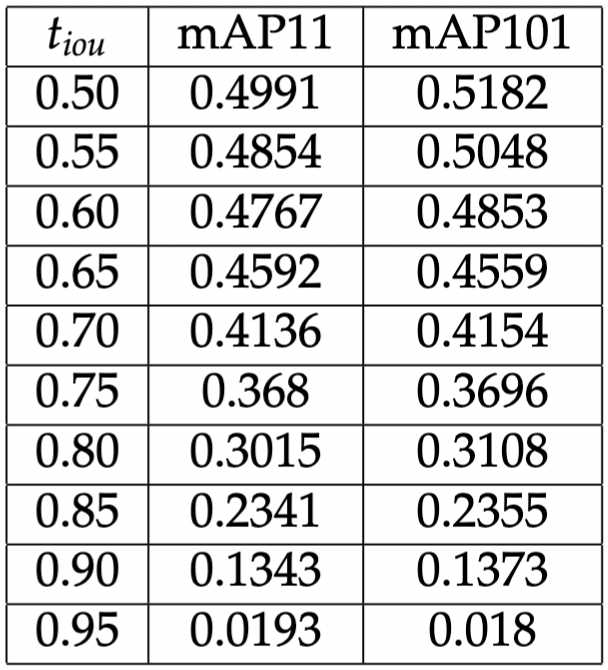
\includegraphics[height=2.25in]{figures/mrcnn_map.png}
    }
    \quad
    \subfloat[][$mAP_{11}$ and $mAP_{101}$ curves]{ 
        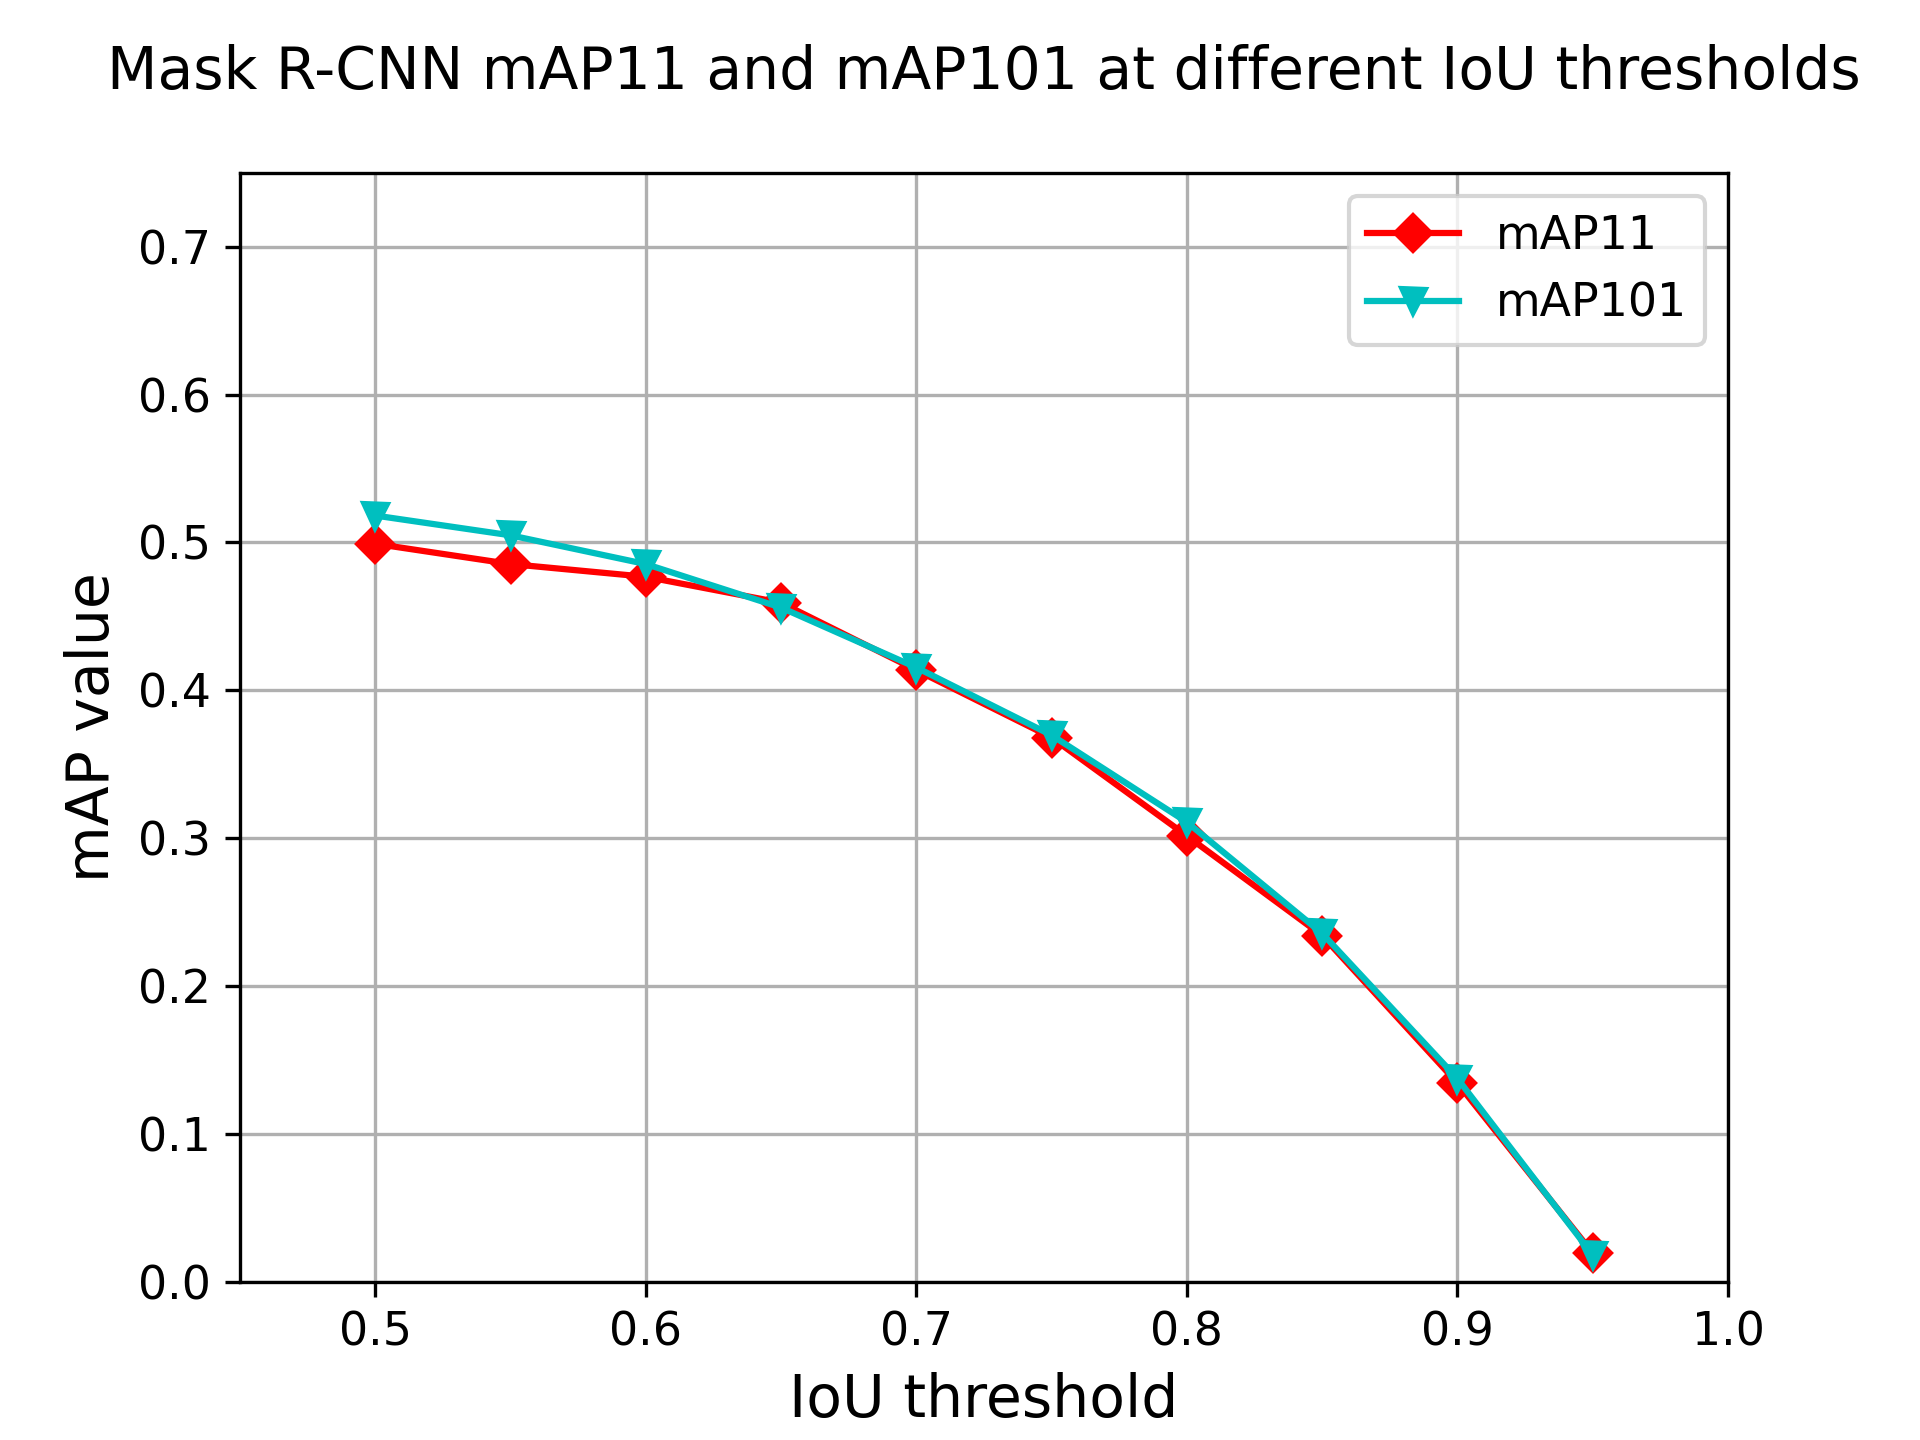
\includegraphics[height=2.25in]{figures/mrcnn_map_curve.png}
    }
    \caption{Mask R-CNN model 11-point interpolation mAP ($mAP_{11}$) and 101-point interpolation mAP ($mAP_{101}$) at different IoU thresholds. The IoU threshold list is defined as [0.5:0.05:0.95], which means the IoU thresholds are from 0.50 to 0.95 with an equal step size of 0.05}  \label{fig:mrcnn_map}
\end{figure}

In contrast to Mask R-CNN, the pre-trained YOLOv5 model only have the $mAP_{101}$ score of 47.18\% at the IoU threshold of 0.5, which indicates that the model is struggling with able to detect the object present in the image. However, YOLOv5 $mAP_{101}$ score gradually decreases as we increase the IoU threshold until 0.85. This means that the YOLOv5 detector is strong in localization task with the majority of predicted bounding boxes, that has IoU larger than 0.5, will have an IoU score of 0.85 approximately.

\begin{figure}[!ht]
    \centering
    \subfloat[][$mAP_{11}$ and $mAP_{101}$ values]{
        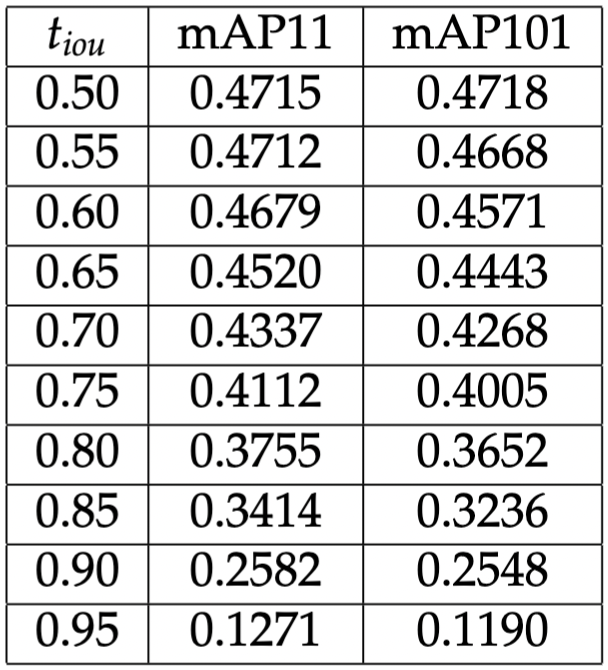
\includegraphics[height=2.25in]{figures/yolov5_map.png}
    }
    \quad
    \subfloat[][$mAP_{11}$ and $mAP_{101}$ curves]{ 
        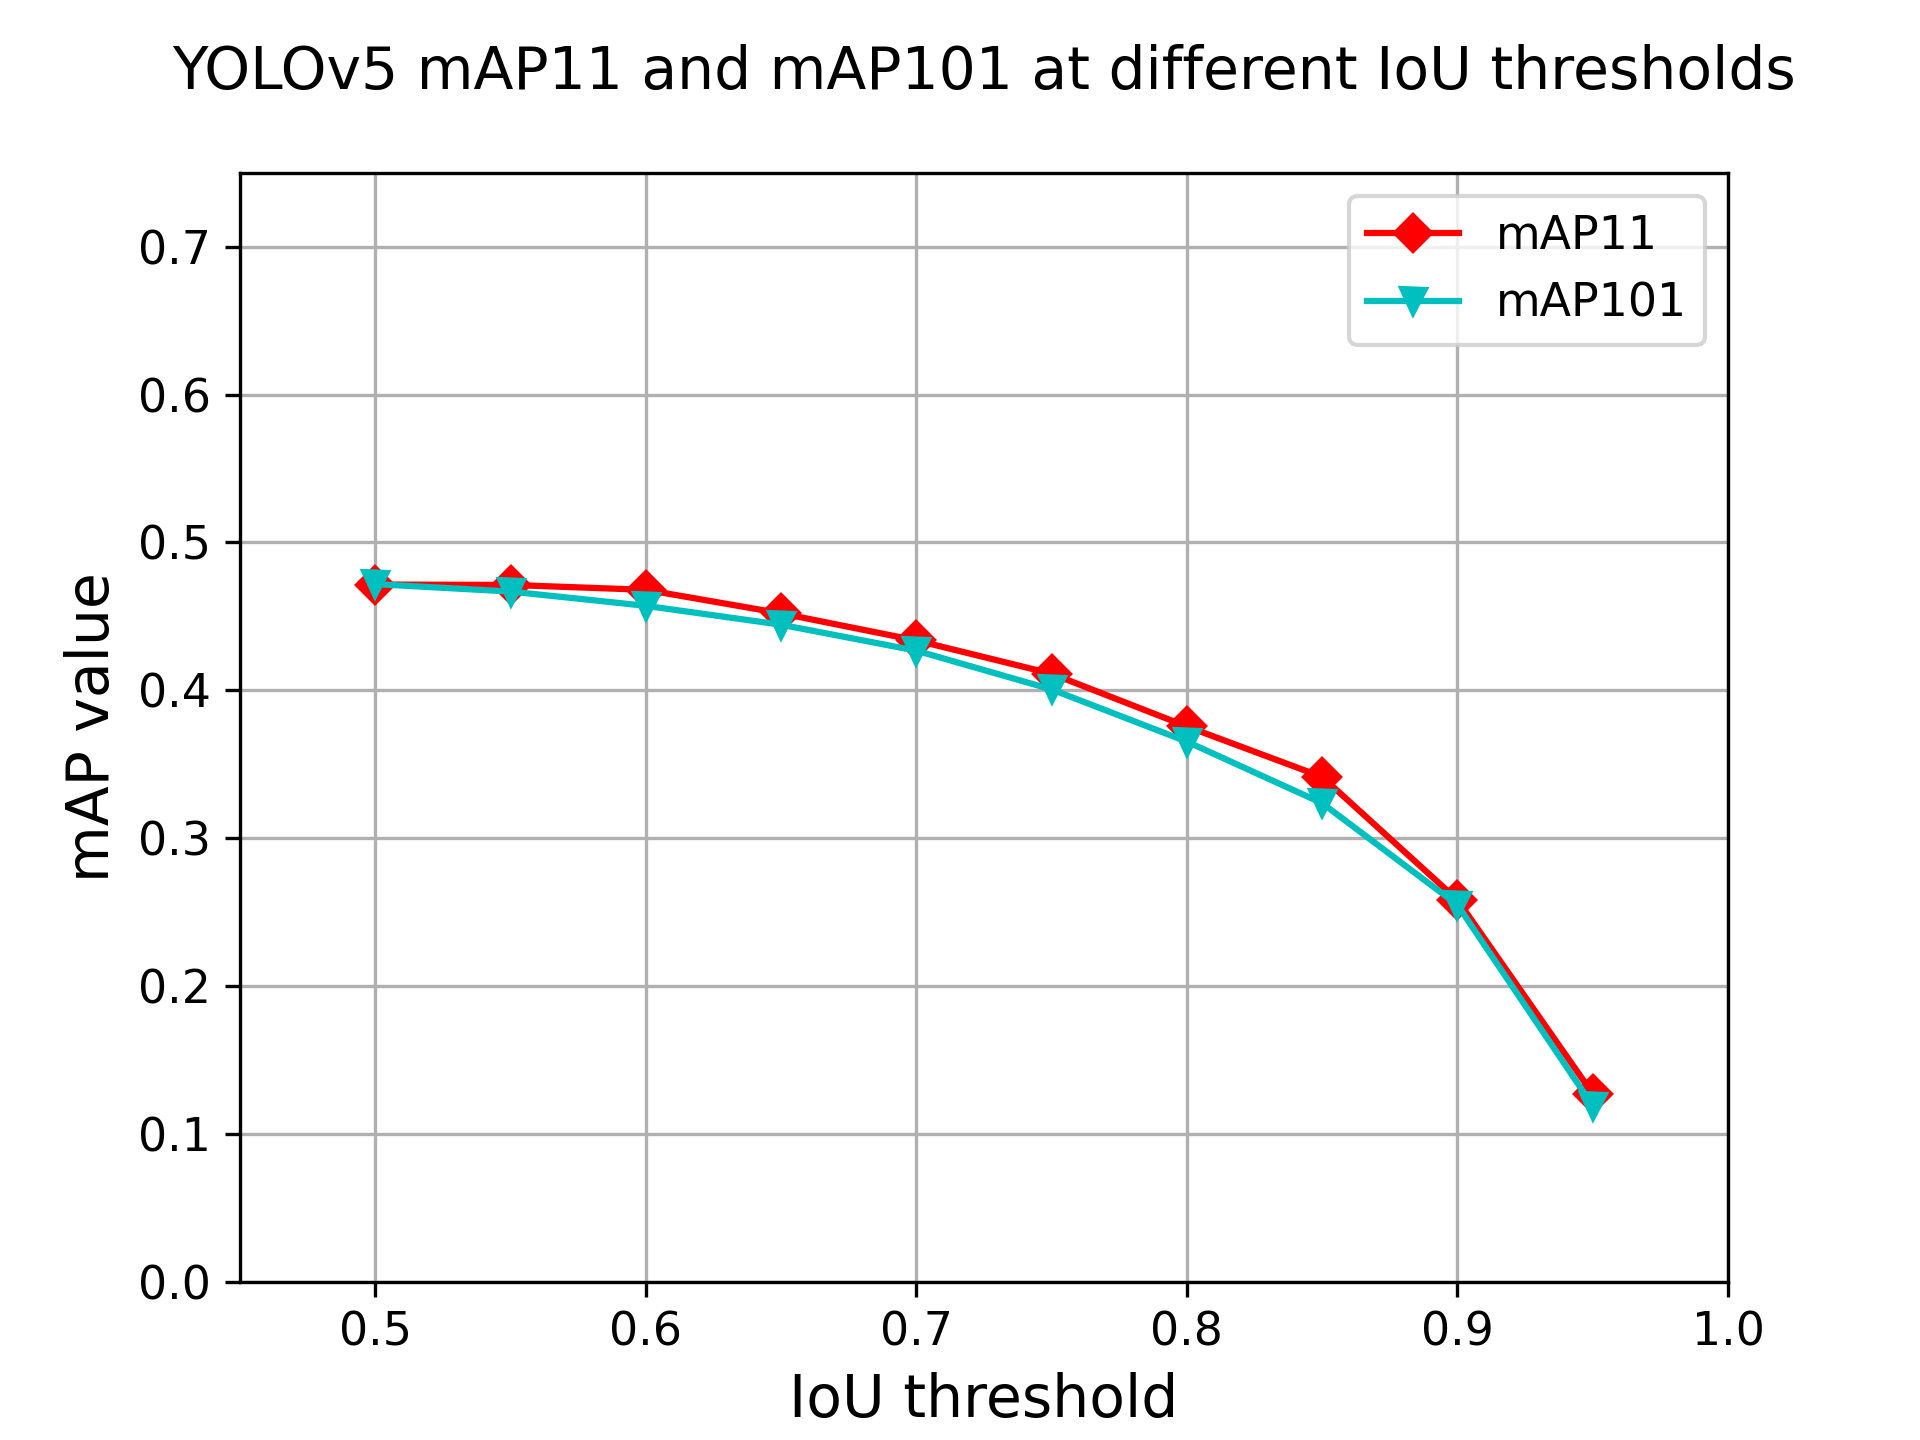
\includegraphics[height=2.25in]{figures/yolov5_map_curve.png}
    }
    \caption{YOLOv5 model 11-point interpolation mAP ($mAP_{11}$) and 101-point interpolation mAP ($mAP_{101}$) at different IoU thresholds. The IoU threshold list is defined as [0.5:0.05:0.95]}  \label{fig:yolov5_map}
\end{figure}

By comparing the $mAP_{101}$ score of the Mask R-CNN and YOLOv5 models, we can clearly see that Mask R-CNN is better at detecting the presence of objects compared to YOLOv5; however, it has a poor localization performance. With poor localization, many detections made by Mask R-CNN are considered as wrong (False Positive) as the IoU threshold increase, and thus reduce the overall $mAP_{101}$ score significantly. On the other hand, YOLOv5, with the high accuracy localization, becomes a better detection model as the IoU threshold approaches 1 (Figure \ref{fig:mrcnn_yolov5_map}). Therefore, for autonomous vehicle applications where both objectiveness and localization are important, YOLOv5 is a better-suited model compared to the Mask R-CNN model. In addition to $mAP_{101}$ score, the breakdown $AP_{101}$ score for each class of the two models at IoU thresholds of 0.55, 0.65, 0.75, and 0.85 are shown in Figure \ref{fig:ap101_perlabel_periou}. Nonetheless, even though YOLOv5 is better compared to Mask R-CNN, at the IoU threshold of 0.85 and confidence threshold of 0.5, YOLOv5 is still unable to detect the majority of ground truth objects. The visualization of the number of missed detection for Mask R-CNN and YOLOv5 model are shown in Figure \ref{fig:model_missed_detection}

\begin{figure}[!ht]
    \centering
    \subfloat[][$mAP_{101}$ values]{
        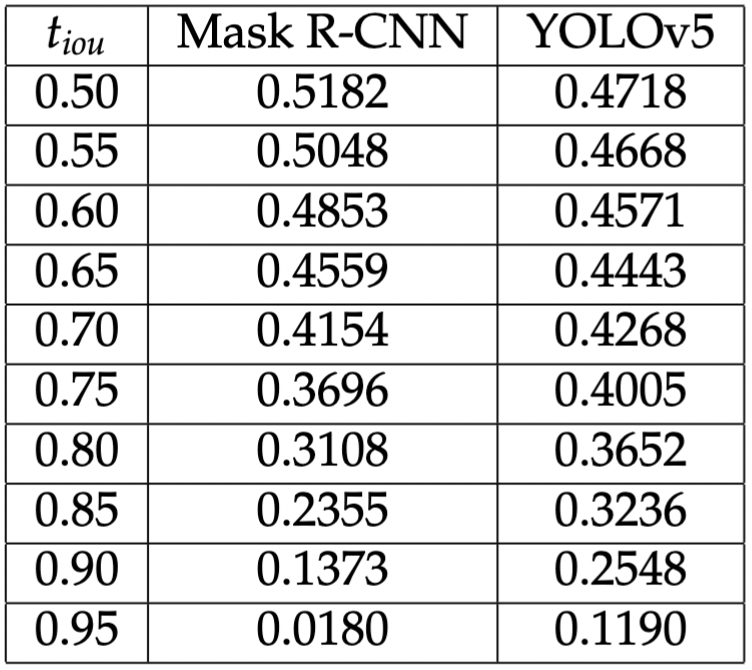
\includegraphics[height=2.25in]{figures/mrcnn_yolov5_map101.png}
    }
    \quad
    \subfloat[][$mAP_{101}$ curves]{ 
        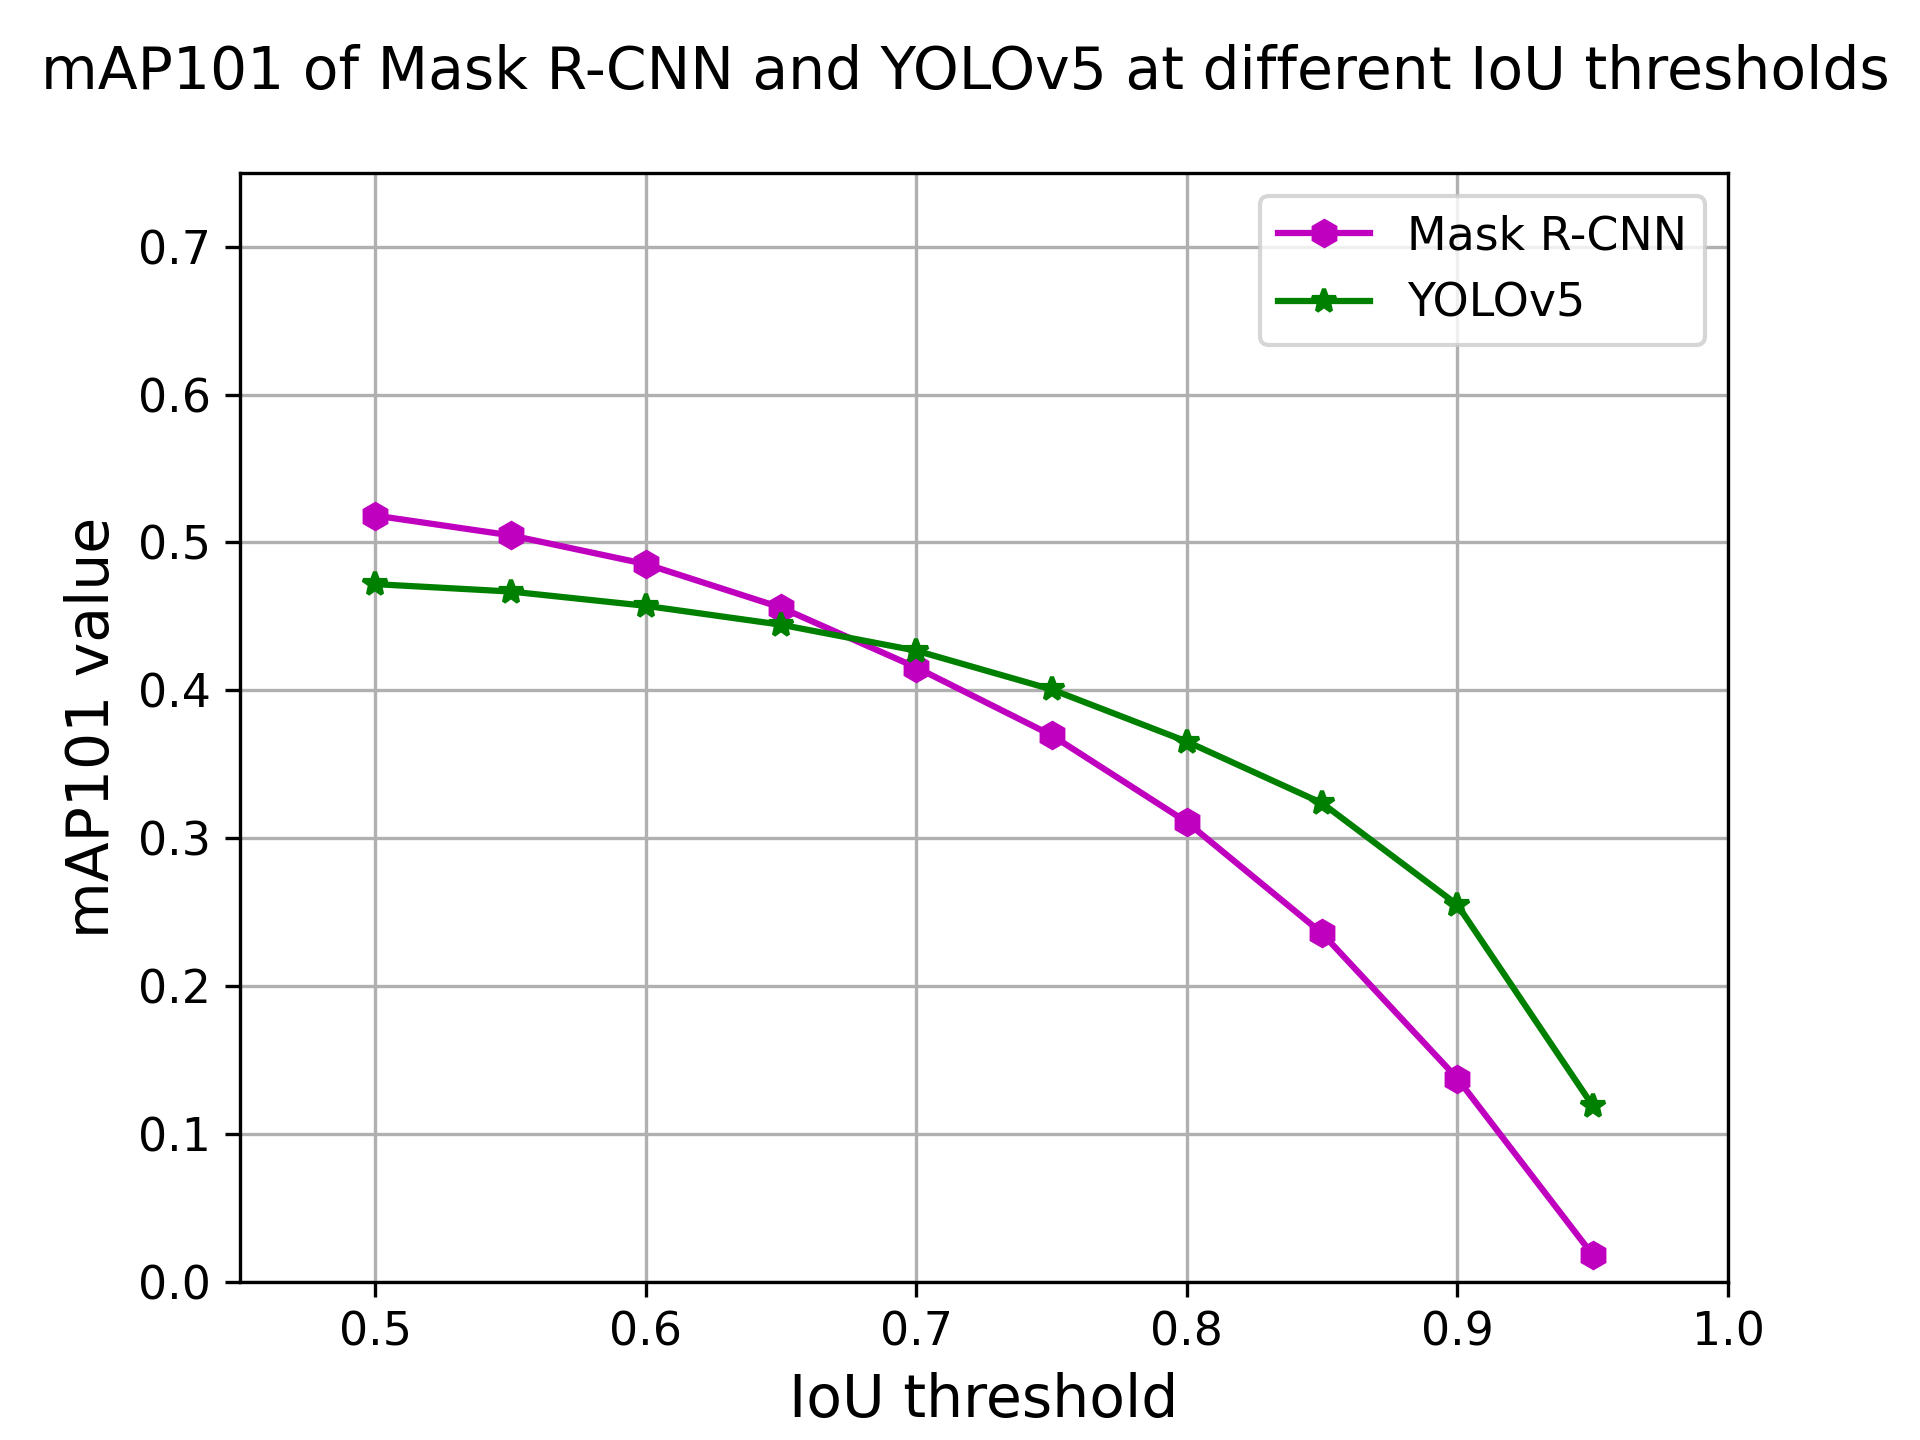
\includegraphics[height=2.25in]{figures/mrcnn_yolov5_map_curve.png}
    }
    \caption{Mask R-CNN's $mAP_{101}$ and YOLOv5's $mAP_{101}$ at different IoU thresholds. The IoU threshold list is defined as [0.5:0.05:0.95]} \label{fig:mrcnn_yolov5_map}
\end{figure}

\begin{figure}[!ht]
    \centering
    \subfloat[][IoU threshold $t_{IoU}=0.55$]{
        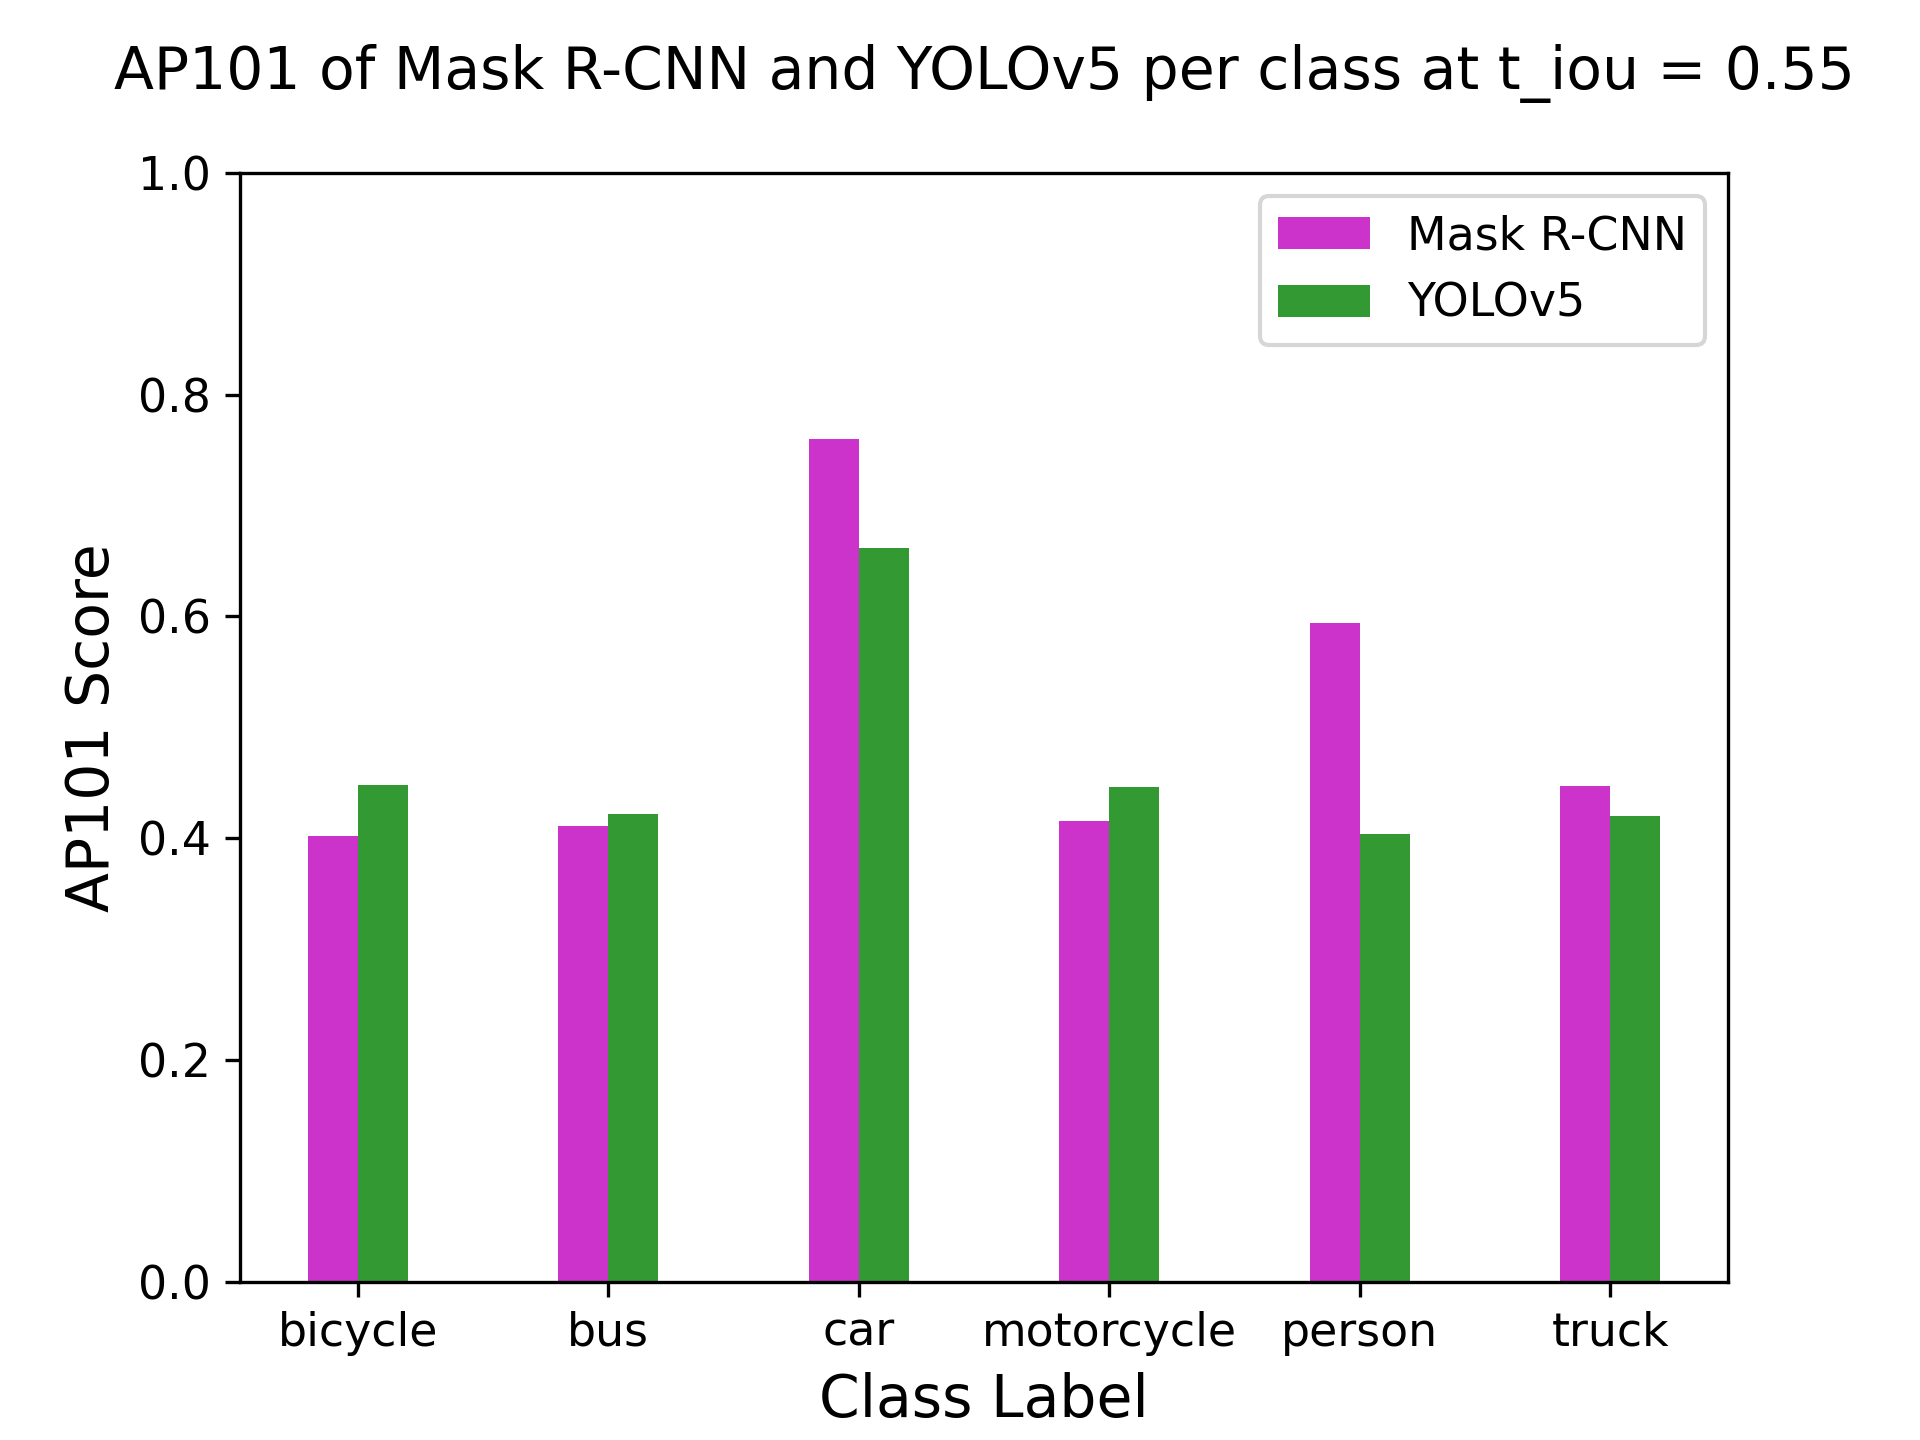
\includegraphics[height=1.5in]{figures/ap101_i55.png}
    }
    \quad
    \subfloat[][IoU threshold $t_{IoU}=0.65$]{
        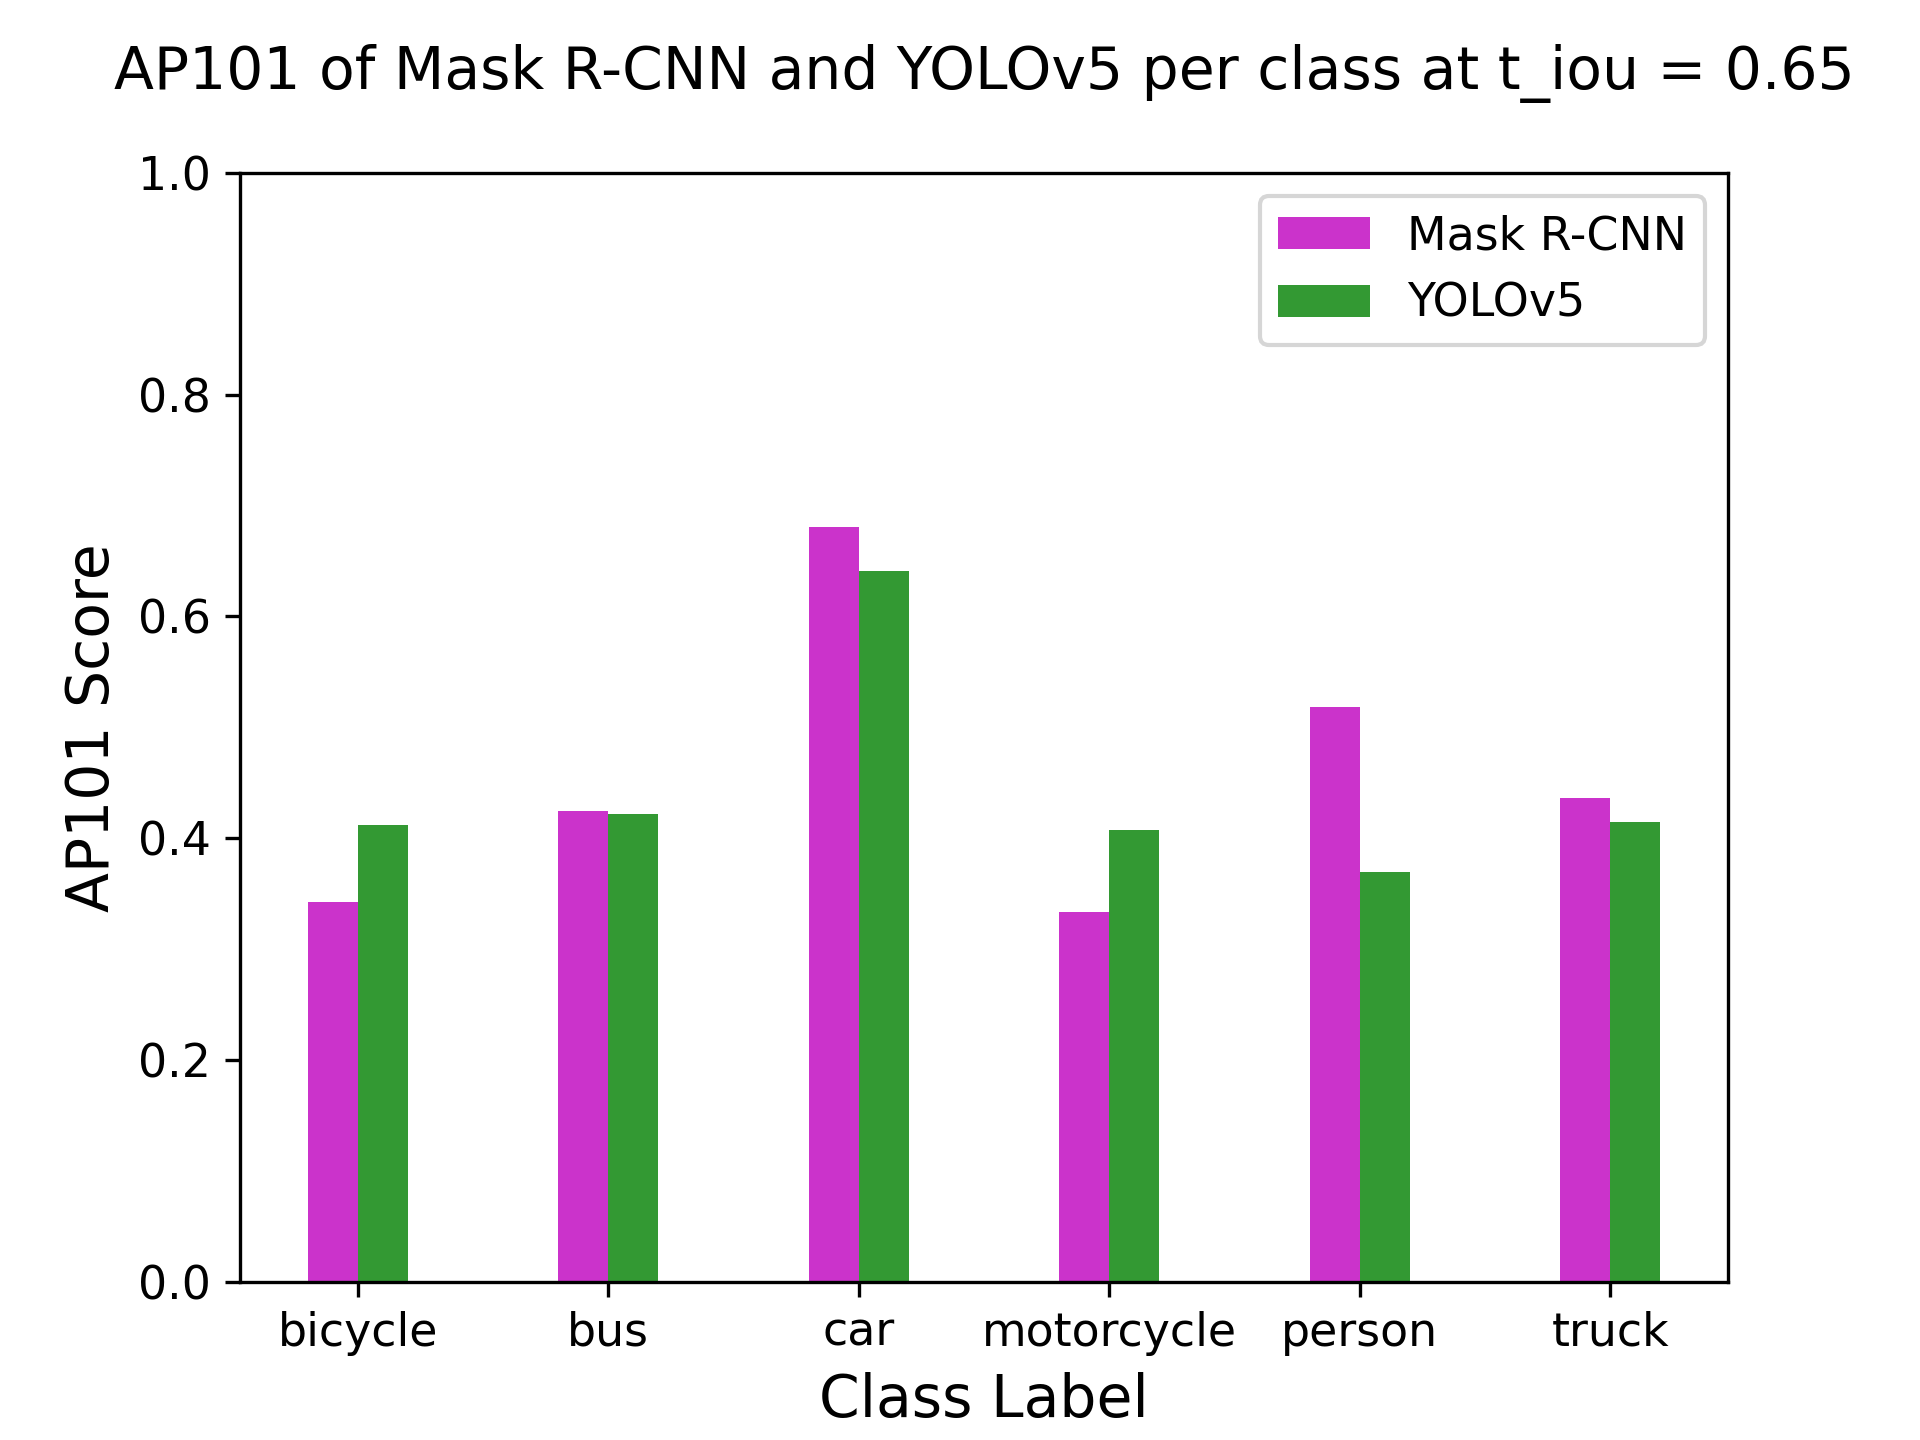
\includegraphics[height=1.5in]{figures/ap101_i65.png}
    }

    \subfloat[][IoU threshold $t_{IoU}=0.75$]{
        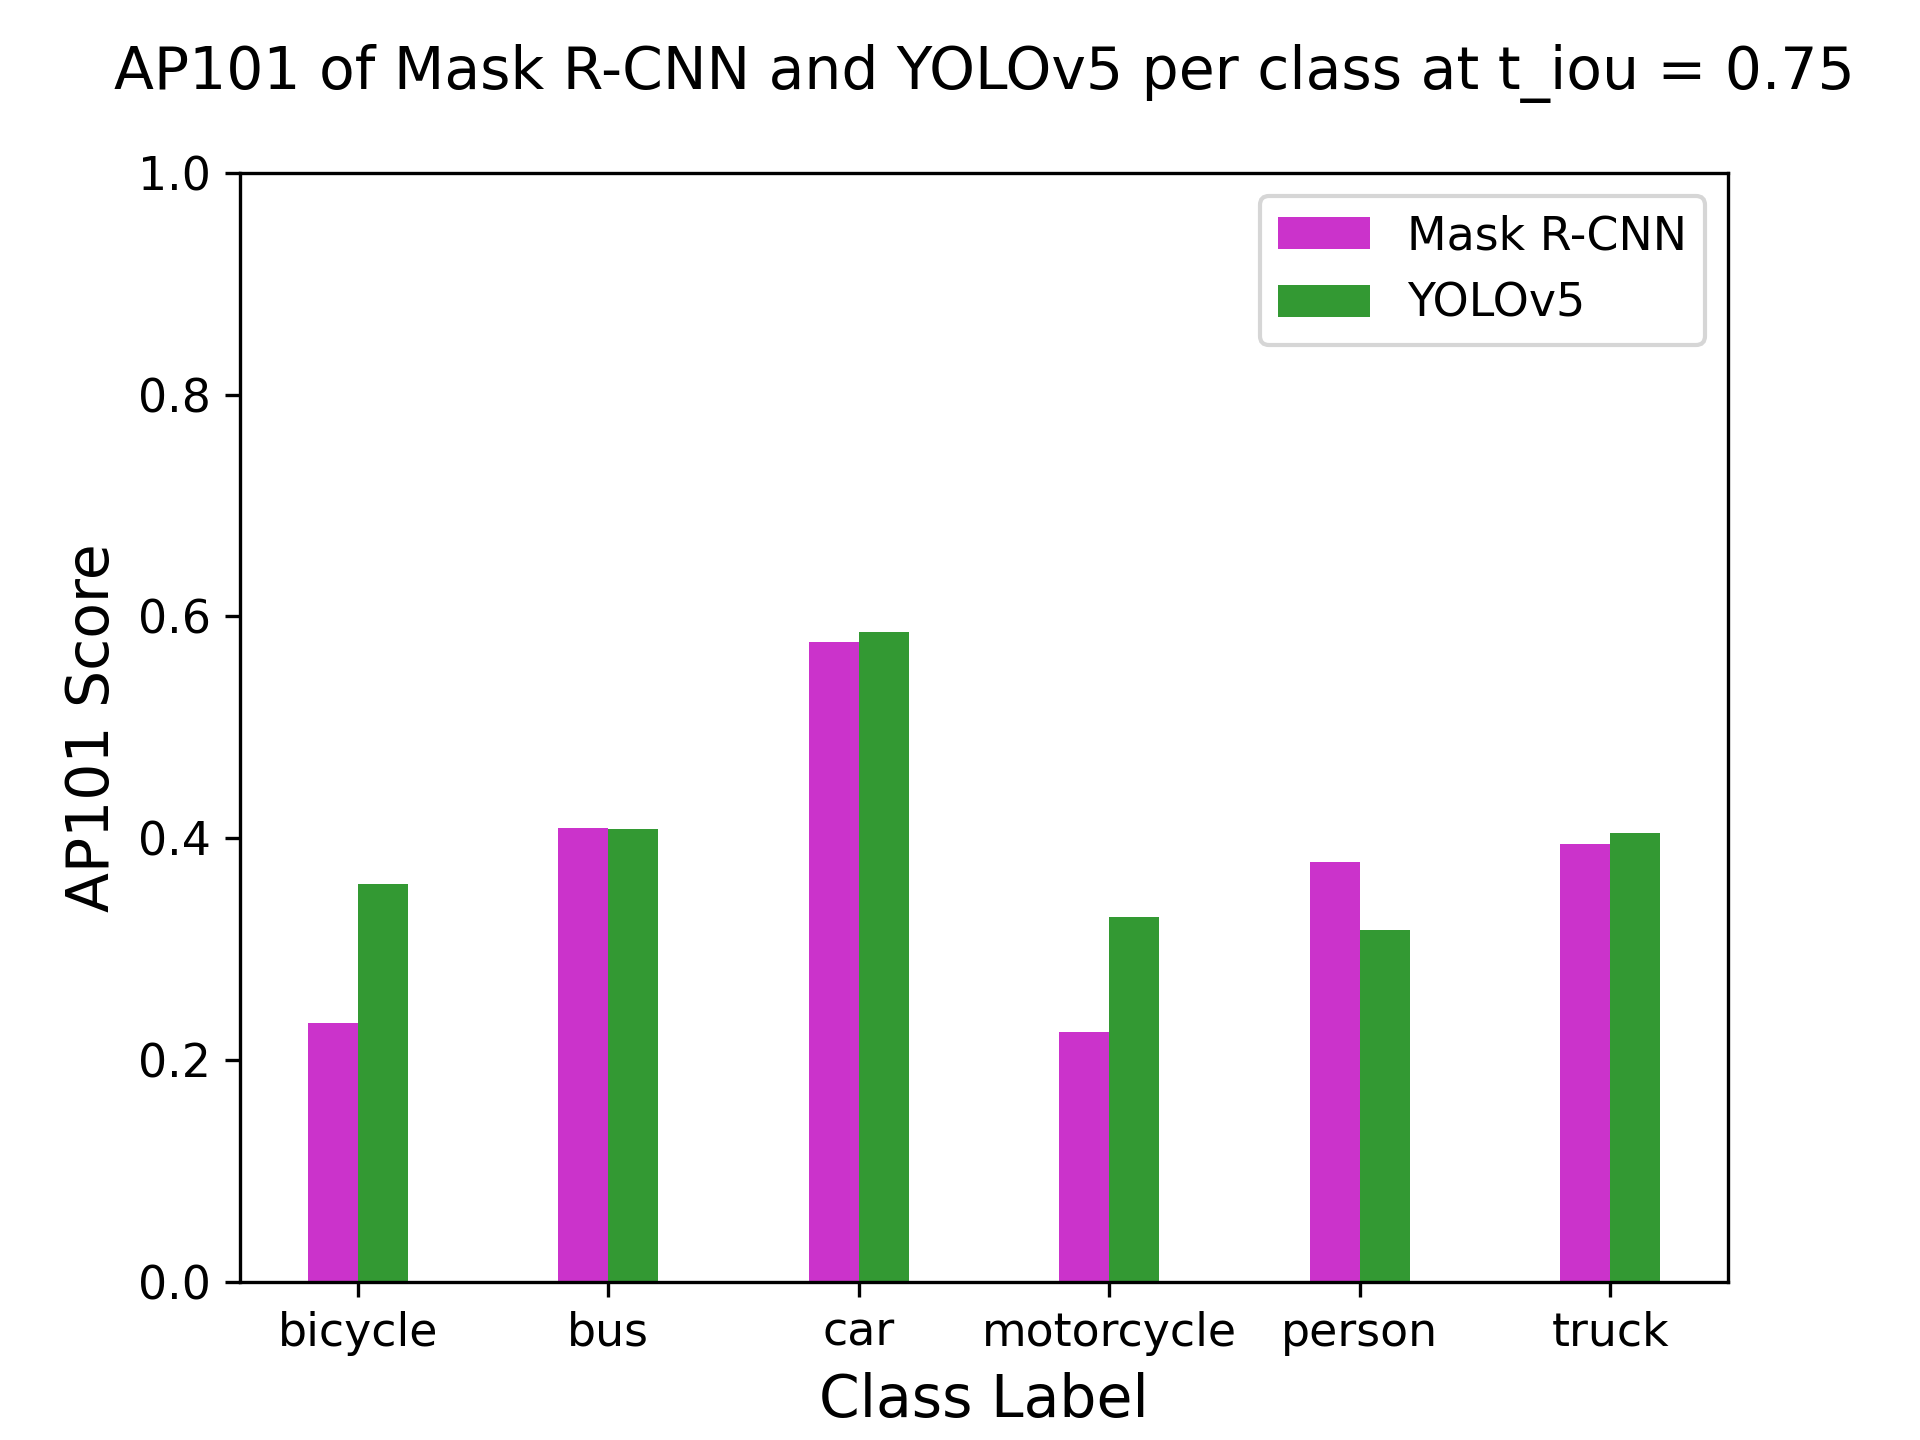
\includegraphics[height=1.5in]{figures/ap101_i75.png}
    }
    \quad
    \subfloat[][IoU threshold $t_{IoU}=0.85$]{
        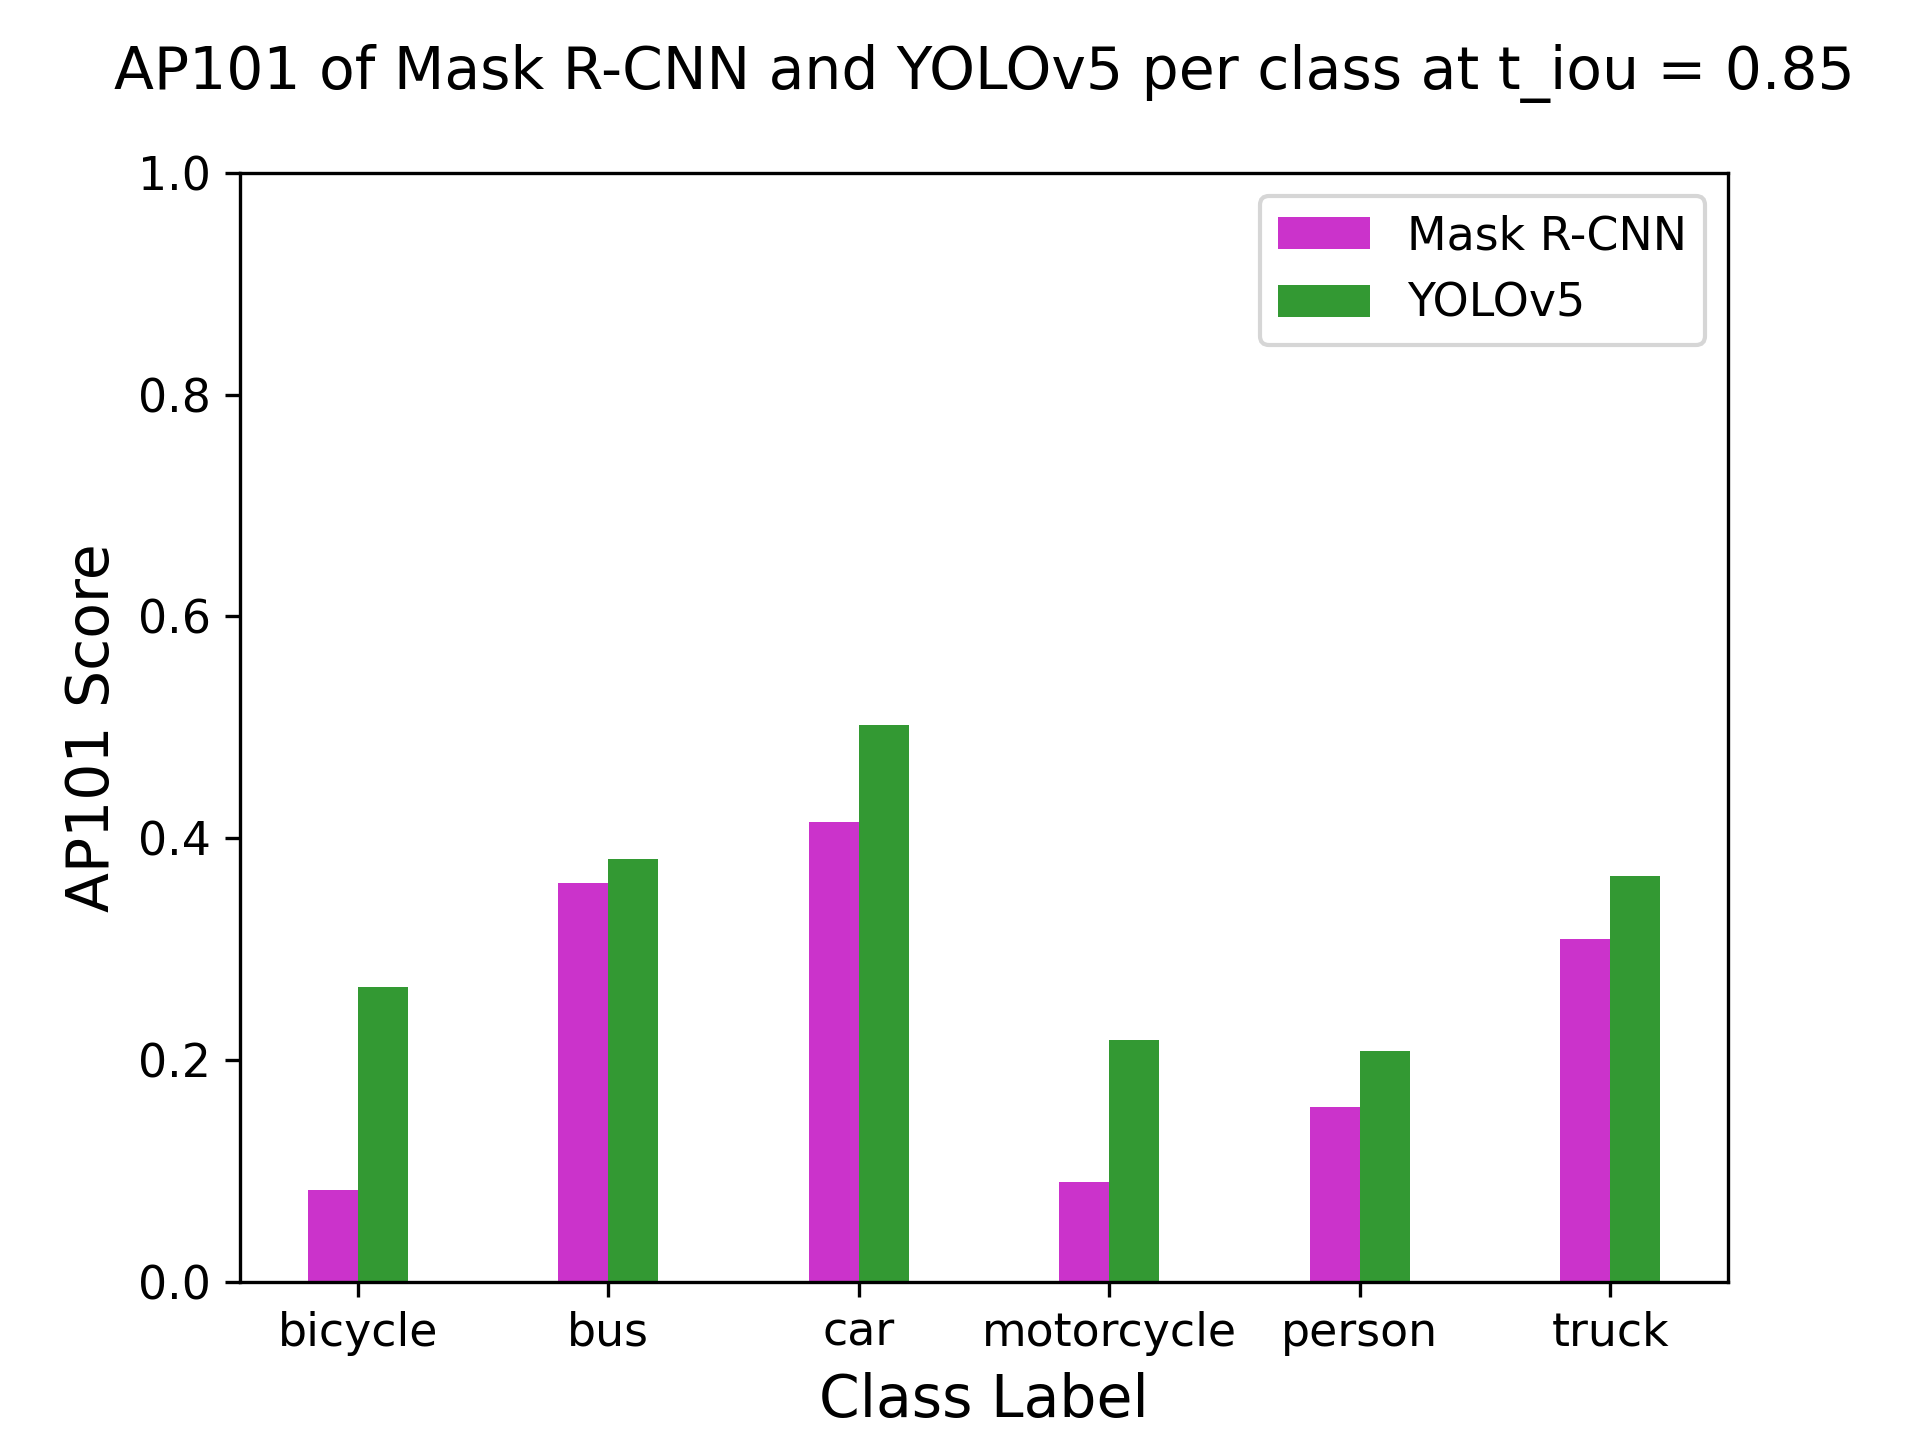
\includegraphics[height=1.5in]{figures/ap101_i85.png}
    }
    \caption{$AP_{101}$ score of Mask R-CNN and YOLOv5 model for each supported label at IoU thresholds of 0.55, 0.65, 0.75, and 0.85} 
    \label{fig:ap101_perlabel_periou}
\end{figure}

\begin{figure}[!ht]
    \centering
    \subfloat[][True Positive at IoU threshold of 0.5 and confidence threshold of 0.5]{
        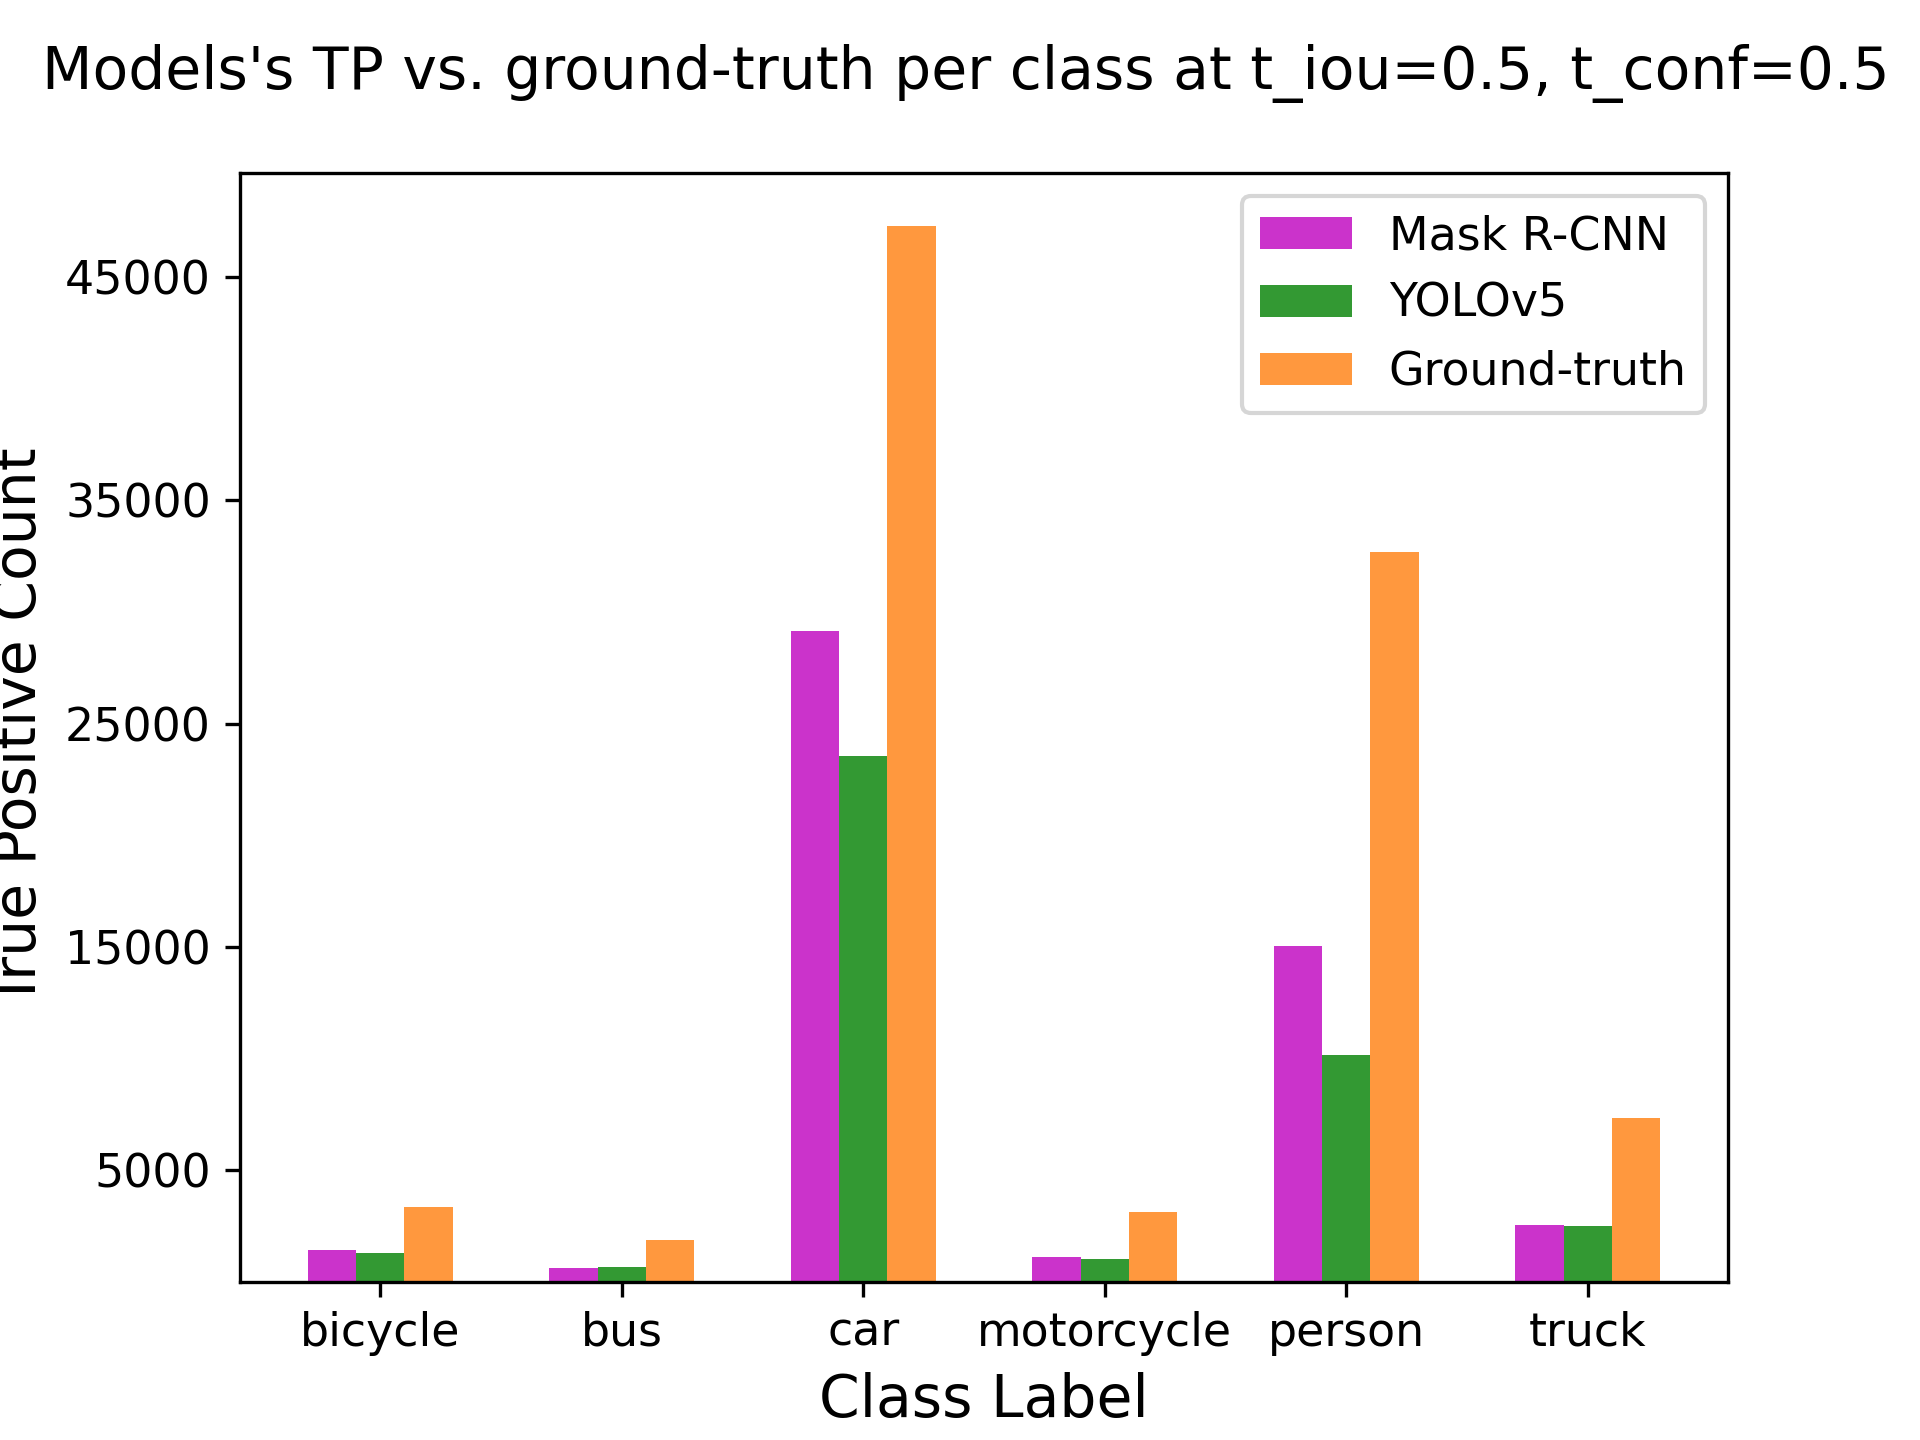
\includegraphics[height=1.5in]{figures/tp_i50_c50.png}
    }
    \quad
    \subfloat[][True Positive at IoU threshold of 0.85 and confidence threshold of 0.5]{ 
        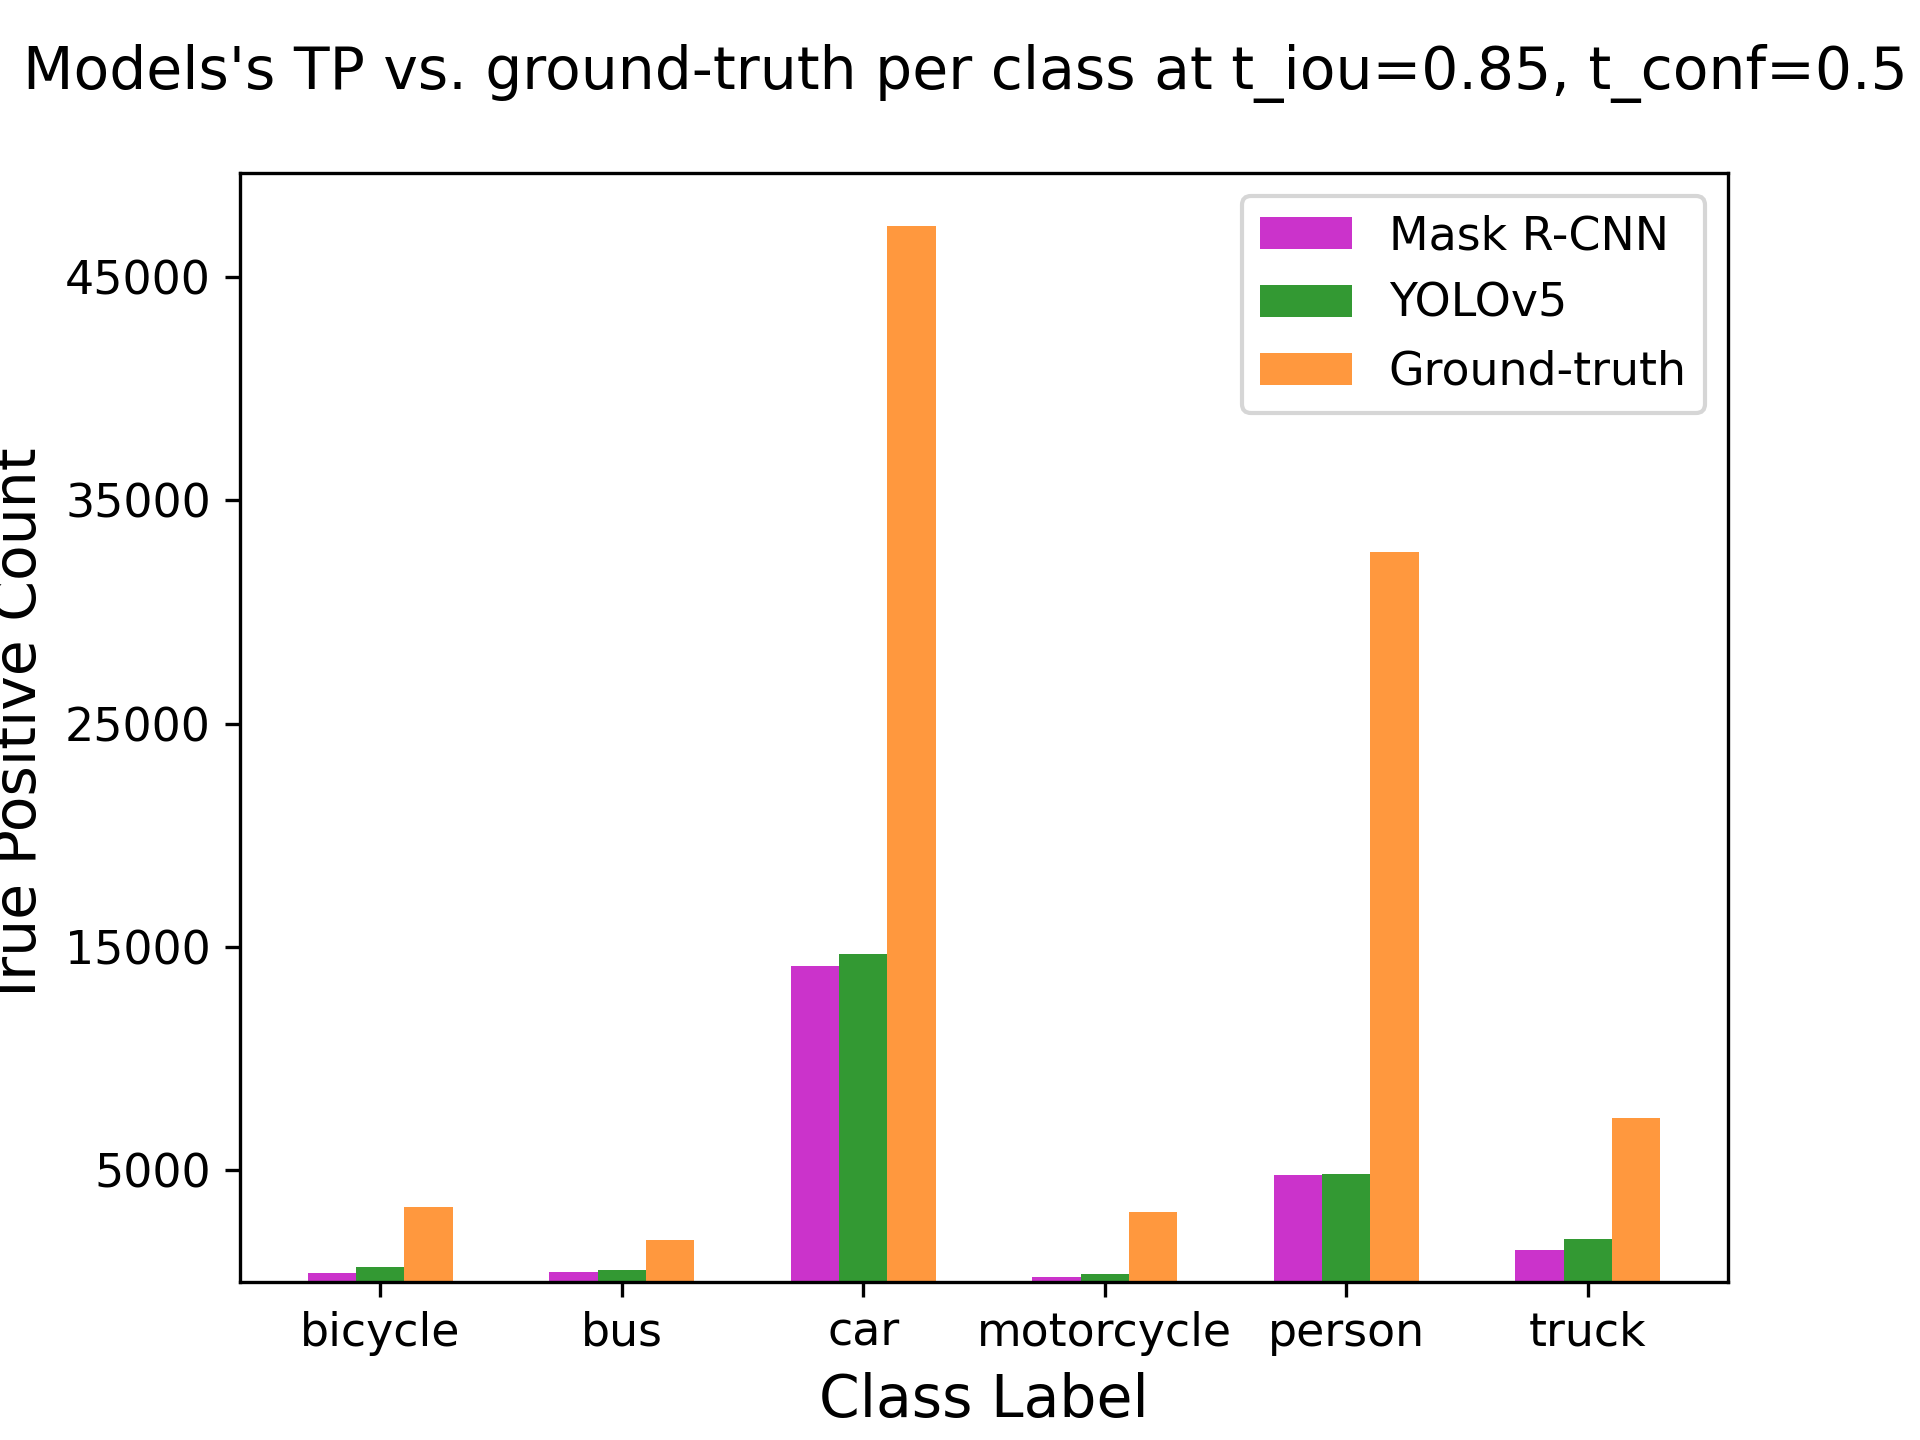
\includegraphics[height=1.5in]{figures/tp_i85_c50.png}
    }
    \caption{Number of detected objects by Mask R-CNN and YOLOv5 versus the number of ground-truth objects. The comparisons are at IoU thresholds of 0.5, 0.85, and the confidence threshold of 0.5. The comparison is displayed for each supported label.} 
    \label{fig:model_missed_detection}
\end{figure}